%; whizzy paragraph -pdf xpdf -latex ./whizzypdfptex.sh
%; whizzy-paragraph "^\\\\begin{frame}\\|\\\\emtext"
% latex beamer presentation.
% platex, latex-beamer でコンパイルすることを想定。 

%     Tokyo Debian Meeting resources
%     Copyright (C) 2012 Junichi Uekawa

%     This program is free software; you can redistribute it and/or modify
%     it under the terms of the GNU General Public License as published by
%     the Free Software Foundation; either version 2 of the License, or
%     (at your option) any later version.

%     This program is distributed in the hope that it will be useful,
%     but WITHOUT ANY WARRANTY; without even the implied warreanty of
%     MERCHANTABILITY or FITNESS FOR A PARTICULAR PURPOSE.  See the
%     GNU General Public License for more details.

%     You should have received a copy of the GNU General Public License
%     along with this program; if not, write to the Free Software
%     Foundation, Inc., 51 Franklin St, Fifth Floor, Boston, MA  02110-1301 USA

\documentclass[cjk,dvipdfmx,12pt]{beamer}
\usetheme{Tokyo}
\usepackage{monthlypresentation}

%  preview (shell-command (concat "evince " (replace-regexp-in-string "tex$" "pdf"(buffer-file-name)) "&")) 
%  presentation (shell-command (concat "xpdf -fullscreen " (replace-regexp-in-string "tex$" "pdf"(buffer-file-name)) "&"))
%  presentation (shell-command (concat "evince " (replace-regexp-in-string "tex$" "pdf"(buffer-file-name)) "&"))

%http://www.naney.org/diki/dk/hyperref.html
%日本語EUC系環境の時
\AtBeginDvi{\special{pdf:tounicode EUC-UCS2}}
%シフトJIS系環境の時
%\AtBeginDvi{\special{pdf:tounicode 90ms-RKSJ-UCS2}}

\newenvironment{commandlinesmall}%
{\VerbatimEnvironment
  \begin{Sbox}\begin{minipage}{1.0\hsize}\begin{fontsize}{8}{8} \begin{BVerbatim}}%
{\end{BVerbatim}\end{fontsize}\end{minipage}\end{Sbox}
  \setlength{\fboxsep}{8pt}
% start on a new paragraph

\vspace{6pt}% skip before
\fcolorbox{dancerdarkblue}{dancerlightblue}{\TheSbox}

\vspace{6pt}% skip after
}
%end of commandlinesmall

\title{東京エリアDebian勉強会}
\subtitle{第128回 2015年7月度}
\author{野島貴英}
\date{2015年7月25日}
\logo{\includegraphics[width=8cm]{image200607/openlogo-light.eps}}

\begin{document}

\begin{frame}
\titlepage{}
\end{frame}

\begin{frame}{設営準備にご協力ください。}
会場設営よろしくおねがいします。
\end{frame}

\begin{frame}{Agenda}
 \begin{minipage}[t]{0.45\hsize}
  \begin{itemize}
   \item 注意事項
	 \begin{itemize}
	  \item 写真はセミナールーム内のみ可です。
          \item 出入りは自由でないので、もし外出したい方は、野島まで一声くださいませ。
	 \end{itemize}
   \item 事前課題発表
  \end{itemize}
 \end{minipage} 
 \begin{minipage}[t]{0.45\hsize}
  \begin{itemize}
   \item 最近あったDebian関連のイベント報告
	 \begin{itemize}
	 \item 第127回 東京エリアDebian勉強会
	 \end{itemize}
   \item Debian Trivia Quiz
   \item DebianでHTTP/2を試す
   \item 今後のイベント
   \item 今日の宴会場所
  \end{itemize}
 \end{minipage}
\end{frame}

\section{事前課題}
\emtext{事前課題}
{\footnotesize
\begin{prework}{ $BLnEg(B }
  \begin{enumerate}
  \item Q.hack time$B$K2?$r$7$^$9$+!)(B\\
    A. $B@-D($j$b$J$/(BNook HD+$B$N(BDebian$B2=!#(B
  \item ($B%*%W%7%g%s(B)Q.$B2?$K$D$$$FJ9$-$?$$!?;22C<T$HOC$r$7$?$$$G$9$+!)(B\\
    A. $B2F5Y$_$K(BDebian$B$G2?$r$9$k!*!)(B
  \end{enumerate}
\end{prework}

\begin{prework}{ issei }
  \begin{enumerate}
  \item Q.hack time$B$K2?$r$7$^$9$+!)(B\\
    A. Hurd$B$r%$%s%9%H!<%k(B
  \end{enumerate}
\end{prework}

\begin{prework}{ wskoka }
  \begin{enumerate}
  \item Q.hack time$B$K2?$r$7$^$9$+!)(B\\
    A. tilegx$B$X$N0\?"(B
  \item ($B%*%W%7%g%s(B)Q.$B$I$3$G:#2s$NJY6/2q$N3+:E$rCN$j$^$7$?$+!)(B\\
    A. $B$=$NB>(B
  \end{enumerate}
\end{prework}

\begin{prework}{ dictoss }
  \begin{enumerate}
  \item Q.hack time$B$K2?$r$7$^$9$+!)(B\\
    A. jessie$B$GF0:n3NG'MQ$N(Blxc$B%3%s%F%J$r:n$C$FF0$+$7$F$_$k(B
  \item ($B%*%W%7%g%s(B)Q.$B$I$3$G:#2s$NJY6/2q$N3+:E$rCN$j$^$7$?$+!)(B\\
    A. Twitter (\@debianjp)
  \end{enumerate}
\end{prework}

\begin{prework}{ nametake }
  \begin{enumerate}
  \item Q.hack time$B$K2?$r$7$^$9$+!)(B\\
    A. Debian$B4D6-9=C[(B
  \item ($B%*%W%7%g%s(B)Q.$B$I$3$G:#2s$NJY6/2q$N3+:E$rCN$j$^$7$?$+!)(B\\
    A. $B$=$NB>(B
  \end{enumerate}
\end{prework}

\begin{prework}{yy\_y\_ja\_jp}
  \begin{enumerate}
  \item Q.hack time$B$K2?$r$7$^$9$+!)(B\\
    A. DDTSS
  \item ($B%*%W%7%g%s(B)Q.$B2?$K$D$$$FJ9$-$?$$!?;22C<T$HOC$r$7$?$$$G$9$+!)(B\\
    A. DDTSS
  \end{enumerate}
\end{prework}

\begin{prework}{koedoyoshida}
  \begin{enumerate}
  \item Q.hack time$B$K2?$r$7$^$9$+!)(B\\
    A. $B$"$s$I$-$e$a$s$F$C$I$G$S$"$sJT=8(B
  \item ($B%*%W%7%g%s(B)Q.$B$I$3$G:#2s$NJY6/2q$N3+:E$rCN$j$^$7$?$+!)(B\\
    A. $B$=$NB>(B
  \end{enumerate}
\end{prework}


}

\section{イベント報告}
\emtext{イベント報告}

\begin{frame}{第127回東京エリアDebian勉強会}

\begin{itemize}
\item 場所はスクウェア・エニックスさんのセミナルームをお借りしての開催でした。
\item 参加者は6名でした。
\item セミナ内容は野島さんによる「Debianと脆弱性対応のあれこれ」でした。
\item 残りの時間でhack timeを行い、成果発表をしました。
\item 宴会の代わりに、「まいどおおきに食堂」で夕食会をやりました。
\end{itemize} 
  
\end{frame}

\begin{frame}{第127回東京エリアDebian勉強会(つづき)}

 セミナは野島さんより、Debianと脆弱性対応について諸々発表がありました。内容としては、すでに公開されている昨今の件のサマリとなりましたが、会場ではいろいろ議論や、追加の情報をいただくことが出来非常に有意義でした。

 また、debianのセキュリティチームからCVE、他のディストリビューションまでOSSの脆弱性の連絡体制ができているのは、さすが沢山の人に支えられているディストリビューションなだけあると思います。
  
\end{frame}

  
\section{Debian Trivia Quiz}
\emtext{Debian Trivia Quiz}
\begin{frame}{Debian Trivia Quiz}

  Debian の常識、もちろん知ってますよね?
知らないなんて恥ずかしくて、知らないとは言えないあんなことやこんなこと、
みんなで確認してみましょう。

今回の出題範囲は\url{debian-devel-announce@lists.debian.org},
\url{debian-news@lists.debian.org} に投稿された
内容などからです。

\end{frame}

\subsection{問題}

%; whizzy-master ../debianmeetingresume201311.tex
% $B0J>e$N@_Dj$r$7$F$$$k$?$a!"$3$N%U%!%$%k$G(B M-x whizzytex $B$9$k$H!"(Bwhizzytex$B$,MxMQ$G$-$^$9!#(B
%

\santaku
{6/22$B$K$F!"(Bbackport$B$N%A!<%`$,!"FCDj$N>r7o$rK~$?$9%Q%C%1!<%8$r$4$C$=$j>C$7$?$N$O!"$I$N(Bbackports?}
{squeeze-backports}
{wheezy-backports}
{jessie-backports}
{B}
{jessie$B$GMxMQ$G$-$J$$%Q%C%1!<%8$r!"(Bwheezy-backports$B$+$i$4$C$=$j>C$7$?$H$N$3$H$G$9!#(Bbackports$B$K4^$^$l$k$I$N%Q%C%1!<%8$,$I$&$J$C$F$$$k$+!)$I$&$7$FM_$7$$$+!)$K$D$$$F$O!"(Bfreeze$B$N4|4V$H(Bfreeze$B8e$N$o$:$+$J4|4V$N4V$K!"(Bbackport$BC4Ev$+$i(Bbackports$B%A!<%`$K<+H/E*$K%?%$%`%j!<$KAjCL$7$FMh$FM_$7$$$H$N4+9p$b9T$o$l$^$7$?!#(B}

\santaku
{7/7$B$K$F!"(Bsid$B$G$O!"FCDj%P!<%8%g%s$N(BGCC$B$H(Blibstdc++$B$G%3%s%Q%$%k!&F0:n=PMh$k$h$&$K$7$FM_$7$$;]$N%"%J%&%s%9$,N.$l$^$7$?!#$I$NAH$_9g$o$;!)(B}
{gcc 6/libstdc++6}
{gcc 4/libstdc++5}
{gcc 5/libstdc++6}
{C}
{$B$^$:$O!"(BDebian sid$B$G$O!"(Bgcc 5/libstdc++6$B$G%3%s%Q%$%k!&F0:n=PMh$k$h$&$K%Q%C%1!<%8%a%s%F%J$NJ}$O=$@5BP1~$r$7$FM_$7$$;]$N%"%J%&%s%9$,$"$j$^$7$?!#:#2s!"(BABI$B%Y!<%9$G$bJQ99$K$J$C$?$j!"(BC++11$B$KBP1~$H$J$C$?$j$G1F6A$,=t!9H/@8$7$^$9!#$^$?!"$3$N1F6A$G!"(BGFortran$BB&$b(Bmodule 14$B$X0\9T$H$J$k$N$G!"(BGFortran$B$r;H$C$F$$$k%Q%C%1!<%8%a%s%F%J$bBP1~$,I,MW$H$N$3$H$G$9!#(B}

\santaku
{7/8$B$K$F!"J#?t$N(Bupstream$B$+$iDs6!$5$l$F$$$k(Blibav*$B72$N%i%$%V%i%j$K$D$$$F!"Ds6!85$N(Bupstream$B$rJQ99$9$k$H$NO"Mm$,$"$j$^$7$?!#$I$N(Bupstream$B$KJQ99$H$J$C$?$N$G$7$g$&$+!)(B}
{FFmpeg}
{libav.org}
{VideoLAN}
{A}
{libav*$B$H$$$&%^%k%A%a%G%#%"$N%G!<%?$r07$&%i%$%V%i%j$J$N$G$9$,!"0lC6(Blibav.org$B$,Ds6!$7$F$$$k$b$N$KJQ99$H$J$C$?$N$G$9$,!"$^$?(BFFmpeg$B$,Ds6!$7$F$$$k$b$N$KLa$C$F$-$?>u67$G$9!#5DO@$N%5%^%j$O(B https://wiki.debian.org/Debate/libav-provider/ffmpeg}

\santaku
{DPL$B$N(BNeil MacGovern$B$,(Breddit$B$K3+$$$?!V(BDPL$B$@$1$I!"2?$+<ALd$"$k!)!W$H$$$&%9%l$G!"(BDPL$B$K$H$C$F$b@($$$H;W$&%G%#%9%H%j%S%e!<%7%g%s$H$7$F$"$2$i$l$F$?$b$N$O$I$l!)(B}
{$BEvA3(BDebian$B$C$7$g!*(B}
{ArchLinux}
{ubuntu}
{B}
{$B%9%l$N=;?M$N<ALd$K!"(BDPL$B$,(BArchLinux$B$,@($$$HEz$($F$$$^$7$?!#(Bwiki$B$N=<<B$V$j$,$H$K$+$/AG@2$i$7$$$H$N$3$H!#(B}

\santaku
{7/20$B$K(Bdgit$B$N?7$7$$%P!<%8%g%s$N$b$N$,%j%j!<%9$5$l$^$7$?!#$I$N%P!<%8%g%s$K$J$C$?!)(B}
{0.1}
{0.3}
{1.0}
{C}
{Debian$B%"!<%+%$%V$r(Bgit$B$GA`:n$G$-$k%D!<%k$N(Bdgit$B$,(B1.0$B$,%j%j!<%9$5$l$?$H$N$3$H$G$9!#AaB.(Bdebian sid$B$K<}O?$5$l$F$$$^$9!#(Bdgit clone package$BL>$H$9$k$H!"(Bhttps://git.dgit.debian.org/ $B$G4IM}$5$l$F$$$k$b$N$,<j85$K(Bclone$B$5$l$^$9!#(B}

\santaku
{7/21$B$K(B Debian Installer Stretch Alpha 1$B$,%j%j!<%9$5$l$^$7$?!#JQ99E@$O0J2<$N$I$l!)(B}
{UEFI$B%V!<%H$rEk:\(B}
{$B%M%C%H%o!<%/(BIF$B$,(BMAC$B%"%I%l%9$K$J$k(B}
{$B%$%s%9%H!<%k;~$N(BUI$B$,(Btext$B%b!<%I$+$i(Bgraphical$B%b!<%I$K$J$C$?(B}
{C}
{Strech$B$GMxMQ$5$l$k$G$"$m$&!"%$%s%9%H!<%i%W%m%0%i%`$N&A(B1$B$,%j%j!<%9$5$l$^$7$?!#$b$A$m$s!"(BStrech$B$,%j%j!<%9$5$l$?$o$1$G$O$J$$$N$GCm0U!#JQ99E@$O?t!9$"$j!"%G%U%)%k%H$N(BCPU$B%"!<%-%F%/%A%c$,(Bamd64$B$K$J$C$?$j$7$?!#>\$7$/$O(Bdebian-devel-announce$B$r;2>H(B}


\section{DebianでHTTP/2を試す}
\emtext{DebianでHTTP/2を試す}

\begin{frame}{はじめに}

 2015/5にHTTP/2がRFC7540として遂に文章化されました。また、最近でも、ほうぼうでWEBページあるいはサービスについて、HTTP/2の対応度合いについて聞かれるようになってきました\footnote{某有名携帯電話イベントでHTTP/2をアプリ開発者に全力推奨している件を見てマヂ慌てたりしたのは秘密...}。

 ここでは、Debianで、HTTP/2の環境をちょっと作って試してみました。

\end{frame}

\begin{frame}{ところでHTTP/2って?(その1)}

  WEBブラウザがサーバと通信する際に、HTTP/1.x(xは0,1の数字)が長年(HTTP/1.1は15年以上も!)使われています。しかしながら、昨今のWEBページは、HTTP/1.xが策定された頃に比べて格段にリッチなページとなっており、1ページを表示する為に必要な通信量は格段に増えています。

\begin{center}
{\Large HTTP/1.xのままでは、WEBの通信が非効率となってしまいました。}
\end{center}

\end{frame}

\begin{frame}{ところでHTTP/2って?(その2)}

  こちらの欠点を克服するために、google社でSPDYが開発され、さらにSPDYを参考にして、沢山の人の貢献により、次世代のHTTP通信規格が策定されました。

\begin{center}
{\Large これがHTTP/2となります。}
\end{center}
    
\end{frame}   

\begin{frame}{HTTP/2の特徴(その1)}

 \begin{itemize}
 \item テキスト電文ベースではなく、バイナリ電文を使います。
 \item 1本のTCPコネクション上で、複数のリクエスト・レスポンスを多重化してやりとりできるように設計されています。
\end{itemize}
   
\end{frame}

\begin{frame}{HTTP/2の特徴(その2)}

 \begin{itemize}
\item  リクエスト・レスポンスに使われるヘッダ情報を無駄の無い電文にし、さらに圧縮し、より効率的に通信できるようにしています。実はモバイル端末などでは、パケットの往復にかかる時間が長いので、リクエスト・レスポンスの開始1パケット目にできるだけ情報を詰め込むことは通信時間を縮めるのに非常に有効です。
 \item 1つのリクエストで、ブラウザが続けて必要とするデータをまとめてレスポンスできる機能が入りました(サーバプッシュという機能。)\\詳しくは「初めてのHTTP/2サーバプッシュ」\url{http://labs.gree.jp/blog/2014/12/11987/}
\end{itemize}
  
\end{frame}

\begin{frame}{HTTP/2さらに詳しく}

  これ以上プロトコルについて、詳しく調べたい人は、

 \begin{itemize}
  \item HTTP/2本家\\
    \url{https://http2.github.io/}
  \item 高速・大規模ネットワーク時代に向けて改良されたHTTP/2プロトコル
    \url{http://www.atmarkit.co.jp/ait/articles/1409/18/news135.html}
  \item twitterの\#http2studyタグ
  \item http/2 Advent Calender 2014
    \url{http://qiita.com/advent-calendar/2014/http2}
\end{itemize}

 などなど、多数ありますので是非。
 \begin{center}
 {\Large Debian勉強会なので、これ以上は割愛!(笑)}
 \end{center}
\end{frame}
  
\begin{frame}{参考:論より証拠}

  論より証拠。どれだけ、HTTP/2が優れているか?を試せる非常に良いデモサイトがあります。是非お試しあれ!(Debian sidのchromium/iceweaselで動作確認済)
  
  \url{https://http2.golang.org/gophertiles}
  
\end{frame}

\begin{frame}{参考:HTTP/2にブラウザでアクセスする時はTLSで}

  HTTP/2を使ってブラウザからアクセスするとき、現状、TLSのALPN/NPNでHTTP/2を指定して、やりとりを開始するやり方しか現行ブラウザには実装されていません。というわけで、事実上、HTTP/2のサイトは、全部フルSSL化されている状況となります。\\
  参考:wikipedia HTTP/2 \\
    \url{https://ja.wikipedia.org/wiki/HTTP/2}

\end{frame}

\begin{frame}{参考:HTTP/2に非TLSでアクセスする方法}
    
  TLSを使わない場合、HTTP/1.1のリクエストヘッダに特別なヘッダを混ぜることにより、HTTP/2へアップグレードして、以降HTTP/2でやり取りをするという手法もありますが、残念ながらブラウザが対応していません。\\

  参考:HTTP/2 プロトコルネゴシエーション方法と ATS での実装\\
  \url{http://techblog.yahoo.co.jp/infrastructure/http2/ats_http2_pn/}
  
\end{frame}


\begin{frame}{DebianでHTTP/2をお手軽に楽しむには!}

 HTTP/2をお手軽に楽しむには以下の環境を用意します。

 \begin{itemize}
  \item クライアント側準備\\
    chromiumか、iceweasel
  \item サーバー側準備\\
     nghttp2,Apache Traffic Server等など
 \end{itemize}  

\end{frame}

\begin{frame}[containsverbatim]{クライアント側準備(chromium編。その1)}

chromiumをDebianに導入します。
  
\begin{commandlinesmall}
$ sudo apt-get install chromium
\end{commandlinesmall}
% $
次に、chromiumを起動して左隅みに現れる「Apps」$\rightarrow$「Web Store」をアクセスし、「HTTP/2 and SPDY indicator」を導入してください。

\end{frame}

\begin{frame}{クライアント側準備(chromium編。その2)}

以上の操作を行ったchromiumでHTTP/2対応のサイトにアクセスすると、青い稲妻マークがアドレスバーに表示されるようになります。

\begin{figure}[H]
\begin{center}
 \includegraphics[width=0.9\hsize]{image201507/chromium-http-2-ready.png}
\end{center}
\caption{HTTP/2のサイトにアクセスした時}
\end{figure}

\end{frame}

\begin{frame}[containsverbatim]{クライアント側準備(iceweasel編。その1)}

iceweaselと、xul-ext-spdy-indicatorをDebianに導入します。
  
\begin{commandlinesmall}
$ sudo apt-get install iceweasel xul-ext-spdy-indicator
\end{commandlinesmall}
% $

\end{frame}

\begin{frame}{クライアント側準備(iceweasel編。その2)}

以上の操作を行ったiceweaselでHTTP/2対応のサイトにアクセスすると、青い稲妻マークがアドレスバーに表示されるようになります。

\begin{figure}[H]
\begin{center}
 \includegraphics[width=0.9\hsize]{image201507/iceweasel-http-2-ready.png}
\end{center}
\caption{HTTP/2のサイトにアクセスした時}
\end{figure}
  
\end{frame}

\begin{frame}{HTTP/2に対応しているサーバ}

  どんなサーバがHTTP/2に対応しているかは、\\
  Implementations \\
  \url{https://github.com/http2/http2-spec/wiki/Implementations}\\
  を参照ください。

\end{frame}

\begin{frame}[containsverbatim]{サーバ側準備(nghttp2 その1)}

 Debian sidにて、HTTP/2対応サーバとして、nghttp2があります。

 \begin{commandlinesmall}
$ sudo apt-get install nghttp2 ssl-cert
\end{commandlinesmall}
% $
 
\end{frame}

\begin{frame}[containsverbatim]{サーバ側準備(nghttp2 その2)}

  ここでは、groffの付属htmlマニュアルをドキュメントルートにしたHTTP/2サーバを立ててみます。

  なお、*-snakeoil.*というファイルは、ssl-crtパッケージを導入すると勝手に作成される自己証明書ファイルとなります。
  
\begin{commandlinesmall}
$ sudo nghttpd -D -d /usr/share/doc/groff-base/html/ \
  443 /etc/ssl/private/ssl-cert-snakeoil.key \
  /etc/ssl/certs/ssl-cert-snakeoil.pem
\end{commandlinesmall}  
%$


\end{frame}

\begin{frame}{実際にHTTP/2でアクセスしてみる}

 早速、先ほど用意したブラウザで、アクセスしてみます。\\
 アクセス先:\url{https://localhost/pic-6.html}
 
\end{frame}

\begin{frame}{chromiumの結果}

\begin{figure}[H]
\begin{center}
 \includegraphics[width=0.9\hsize]{image201507/chromium-groff-access.png}
\end{center}
\caption{chromiumでアクセス}
\end{figure}
 
\end{frame}

\begin{frame}{iceweaselの結果}

\begin{figure}[H]
\begin{center}
 \includegraphics[width=0.9\hsize]{image201507/iceweasel-groff-access.png}
\end{center}
\caption{iceweaselでアクセス}
\end{figure}
 
\end{frame}

\begin{frame}{結果}
\begin{center}  
{\LARGE 無事HTTP/2でアクセスできてます。}
\end{center}  
\end{frame}  

\begin{frame}{proxyサーバで既存サイトのHTTP/2化をやってみる}

 さて、nghttpdは軽量のHTTP/2対応WEBサーバではあるのですが、やっぱりapacheのような高機能なWEBサーバを使ってHTTP/2を実現したいというニーズがあると思います。(例:phpのサイトをHTTP/2化したい等)

 今度は、apacheをバックエンドにして、nghttp2付属のproxyサーバを使い、サイトのHTTP/2化を行ってみます。
  
\end{frame}  

\begin{frame}{概念図}

\begin{figure}[H]
\begin{center}
 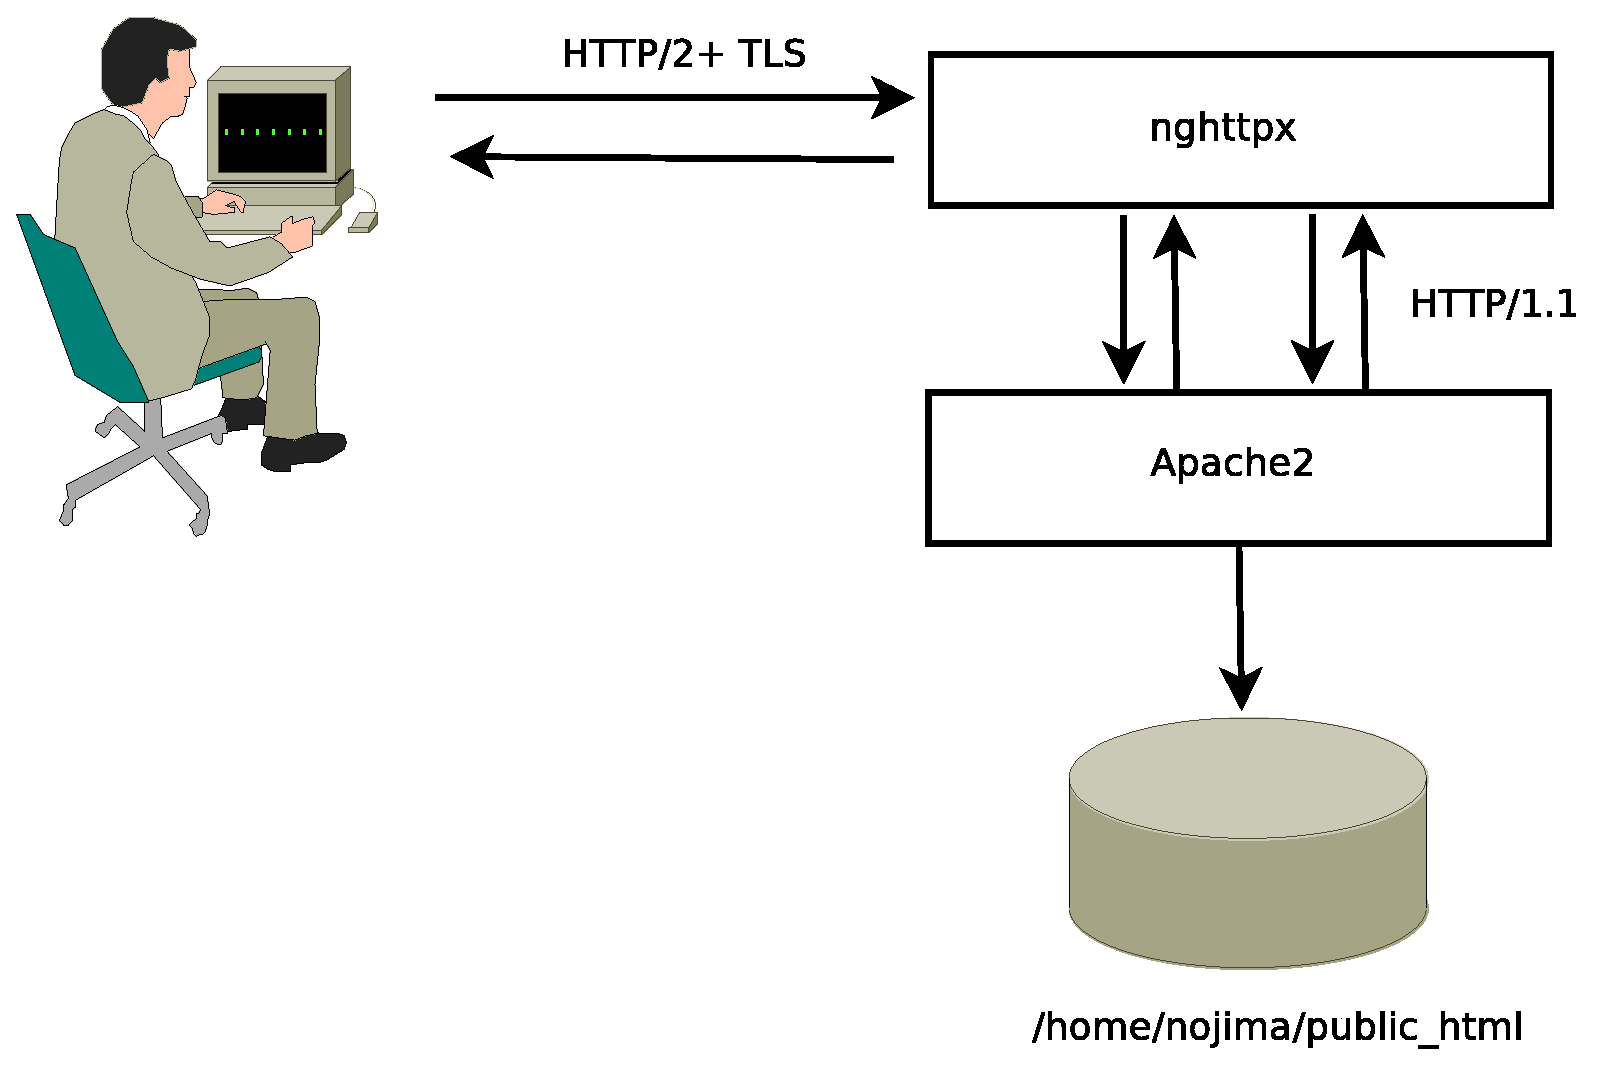
\includegraphics[width=1.0\hsize]{image201507/nghttpx-apache-proxying.eps}
\end{center}
\caption{proxyサーバでHTTP/2化やってみる}
\end{figure}
  
\end{frame}    

\begin{frame}{proxyサーバでHTTP/2やってみる(その1)}

 手順:\\
\begin{description}
\item [Step 1.] sudo apt-get install apache2 nghttp2 ssl-cert
\item [Step 2.] sudo a2enmod userdir
\item [Step 3.] cd /home/yours/; mkdir public\_html
\item [Step 4.] cd public\_html; cp -a /usr/share/doc/groff-base/html .
\end{description}

\end{frame}

\begin{frame}{proxyサーバでHTTP/2やってみる(その2)}

 手順つづき:
\begin{description}
\item [Step 5.] sudo vi /etc/nghttpx/nghttpx.conf\\
  ----nghttpx.confの中身ここから----\\
frontend=0.0.0.0,443 \\
backend=127.0.0.1,80 \\
private-key-file=/etc/ssl/private/ssl-cert-snakeoil.key \\
certificate-file=/etc/ssl/certs/ssl-cert-snakeoil.pem \\
workers=1 \\
  ----ここまで----
\item [Step 6.] sudo systemctl start apache2.service
\item [Step 7.] sudo nghttpx -D --conf /etc/nghttpx/nghttpx.conf
\end{description}

\end{frame}

\begin{frame}{proxyサーバでHTTP/2やってみる(その3)}

 アクセス先:\url{http://localhost/~yours/html/pic.html}\\
\begin{center}
 {\Large 無事 HTTP/2でアクセスできました}
\end{center}

\end{frame}

\begin{frame}{おわりに}

 HTTP/2もDebianを使えば簡単に実験できます。是非おためしあれ!
  
\end{frame}

\section{今後のイベント}
\emtext{今後のイベント}
\begin{frame}{今後のイベント}
\begin{itemize}
 \item 関西エリアDebian勉強会
 \item 東京エリアDebian勉強会(8/22(土)?)
\end{itemize}
\end{frame}

\section{今日の宴会場所}
\emtext{今日の宴会場所}
\begin{frame}{今日の宴会場所}
未定
\end{frame}

\end{document}

;;; Local Variables: ***
;;; outline-regexp: "\\([ 	]*\\\\\\(documentstyle\\|documentclass\\|emtext\\|section\\|begin{frame}\\)\\*?[ 	]*[[{]\\|[]+\\)" ***
;;; End: ***
